\documentclass[11pt,a4paper]{report}
\usepackage{graphicx}
\graphicspath{{./images/}}
\usepackage[utf8]{inputenc}
\usepackage{amsmath}
%\usepackage{tabto}
\usepackage{amsfonts}
\usepackage{amssymb}
\usepackage{amsthm}
\usepackage{xcolor}
\usepackage{setspace}
\usepackage[margin=1in]{geometry}

\usepackage[colorlinks=true,          % link colors, set to 'false' for print version
            linkcolor=blue,
            citecolor=red,
            urlcolor=blue]{hyperref}
\onehalfspacing            
\graphicspath{ {./images/} }

%\setlength{\topmargin}{30mm}
%\addtolength{\topmargin}{-1in}
%\addtolength{\topmargin}{-\headsep}
%\addtolength{\topmargin}{-\headheight}
%\addtolength{\topmargin}{-\topskip}

%\setlength{\textheight}{270mm}
%\addtolength{\textheight}{\topskip}
%\addtolength{\textheight}{-\footskip}
%\addtolength{\textheight}{-30pt}

%\setlength{\oddsidemargin}{-1in}
%\addtolength{\oddsidemargin}{20mm}
%\setlength{\evensidemargin}{\oddsidemargin}

%\setlength{\textwidth}{170mm}

\newtheorem{defn}{Definition}[section]
 \newtheorem{thm}{Theorem}[section]
 \newtheorem{Lemma}{Lemma}[section]
 \newtheorem{Claim}{Claim}[section]
 \newtheorem{Prop}{Proposition}[section]
  \theoremstyle{definition}\newtheorem{Ex}{Example}[section]
 \newtheorem{Cor}{Corollary}[section]
 \newtheorem{claim}{Claim}[section]
 \newtheorem{conj}{Conjecture}  

\usepackage {amsfonts,amssymb}
%\usepackage{mathbbol}
\usepackage{latexsym}
\usepackage{mathrsfs}
\input xy
\xyoption{all}

\newcommand {\op}{\mathcal{O}\mathfrak{p}}
\newcommand {\Def}{\textrm{Def}}
\newcommand {\MC} {\textrm{MC}}
\newcommand {\Art}{\textrm{Art}_\CC}
\newcommand {\Kur}{\textrm{Kur}}
\newcommand {\LG} {^LG}
\newcommand{\fart}{\textrm{FArt}_\CC}
\newcommand{\fun}{\textrm{Fun}}
\newcommand{\sets}{\textrm{Sets}}
\newcommand{\tops}{\textrm{Top}}

\newcommand {\BB}{\mathbb{B}}
\newcommand {\CC}{\mathbb{C}}
\newcommand {\FF}{\mathbb{F}}
\newcommand {\KK}{\mathbb{K}}
\newcommand {\MM}{\mathbb{M}}
\newcommand{\NN}{\mathbb{N}}
\newcommand {\PP}{\mathbb{P}}
\newcommand{\QQ}{\mathbb{Q}}
\newcommand {\RR}{\mathbb{R}}
\newcommand {\SSS}{\mathbb{S}}
\newcommand {\VV}{\mathbb{V}}
\newcommand {\HH}{\mathbb{H}}
\newcommand {\WW}{\mathbb{W}}
\newcommand{\YY}{\mathbb{Y}}
\newcommand{\ZZ}{\mathbb{Z}}


\newcommand {\bal}{\boldsymbol{\alpha}}
\newcommand {\bbe}{\boldsymbol{\beta}}
\newcommand {\bga}{\boldsymbol{\gamma}}
\newcommand {\bmu}{\boldsymbol{\mu}}
\newcommand {\bom}{\boldsymbol{\omega}}
\newcommand {\bth}{\boldsymbol{\theta}}
\newcommand {\bph}{\boldsymbol{\phi}}
\newcommand {\bdh}{\boldsymbol{h}}
\newcommand {\bdk}{\boldsymbol{k}}
\newcommand {\bdE}{\boldsymbol{E}}
\newcommand {\bdU}{\boldsymbol{U}}
\newcommand {\bdP}{\boldsymbol{P}}
\newcommand {\ba}{{\bf a}}
\newcommand {\bb}{{\bf b}}
\newcommand {\bc}{{\bf c}}
\newcommand {\bd}{{\bf d}}
\newcommand {\bg}{{\bf g}}
\newcommand {\be}{{\bf e}}
\newcommand {\bdf}{{\bf f}}
\newcommand {\bp}{{\bf p}}
\newcommand {\bq}{{\bf q}}
\newcommand {\bv}{{\bf v}}
\newcommand {\bh}{{\bf h}}
\newcommand {\bk}{{\bf k}}
\newcommand {\br}{{\bf r}}
\newcommand {\bdu}{{\bf u}}
\newcommand {\bdv}{{\bf v}}
\newcommand {\bi}{{\bf i}}
\newcommand {\bj}{{\bf j}}
\newcommand {\bn}{{\bf n}}
\newcommand {\bs}{{\bf s}}
\newcommand {\bt}{{\bf t}}
\newcommand {\bu}{{\bf u}}
\newcommand {\bw}{{\bf w}}
\newcommand {\bx}{{\bf x}}
\newcommand{\by}{{\bf y}}
\newcommand {\bz}{{\bf z}}
\newcommand {\bB}{{\bf B}}
\newcommand{\bD}{{\bf D}}
\newcommand {\bE}{{\bf E}}
\newcommand {\bF}{{\bf F}}
\newcommand {\bG}{{\bf G}}
\newcommand {\bH}{{\bf H}}
\newcommand {\bK}{{\bf K}}
\newcommand {\bL}{{\bf L}}
\newcommand {\bM}{{\bf M}}
\newcommand {\bN}{{\bf N}}
\newcommand {\bO}{{\bf O}}
\newcommand {\bP}{{\bf P}}
\newcommand {\bQ}{{\bf Q}}
\newcommand {\bR}{{\bf R}}
\newcommand {\bT}{{\bf T}}
\newcommand {\bS}{{\bf S}}
\newcommand {\bU}{{\bf U}}
\newcommand {\bV}{{\bf V}}
\newcommand {\bW}{{\bf W}}
\newcommand {\bgamma}{\boldsymbol\gamma}
\newcommand {\bdelta}{\boldsymbol\delta}
\newcommand {\bDelta}{\boldsymbol\Delta}
%\newcommand{\qed}{{\ \bf qed}}

\newcommand {\rroot}{\mathbf{root}}
\newcommand {\coroot}{\mathbf{coroot}}
\newcommand {\weight}{\mathbf{weight}}
\newcommand {\coweight}{\mathbf{coweight}}
 \newcommand{\higgs}{\textrm{Higgs}}
\newcommand{\bun}{\textrm{Bun}}
\newcommand{\rk}{\textrm{rk}}
\newcommand{\ext}{\textrm{Ext}}
% \newcommand {\id}{\mathbb{1}}
% Use \id if using mathbbol instead of amssymb
\newcommand{\range}{\textrm{Range}}
\newcommand{\arccot}{\textrm{arccot}}

\newcommand{\thickslash}{\mathbin{\!\!\pmb{\fatslash}}}


\newcommand{\cA}{\mathcal{A}}
\newcommand{\cB}{\mathcal{B}}
\newcommand{\cC}{\mathcal{C}}
\newcommand{\cD}{\mathcal{D}}
\newcommand{\cE}{\mathcal{E}}
\newcommand{\cF}{\mathcal{F}}
\newcommand{\cG}{\mathcal{G}}
\newcommand{\cH}{\mathcal{H}}
\newcommand{\cI}{\mathcal{I}}
\newcommand{\cJ}{\mathcal{J}}
\newcommand{\cK}{\mathcal{K}}
\newcommand{\cL}{\mathcal{L}}
\newcommand {\cM}{\mathcal{M}}
\newcommand {\cN}{\mathcal{N}}
\newcommand {\cO}{\mathcal{O}}
\newcommand{\cP}{\mathcal{P}}
\newcommand{\cQ}{\mathcal{Q}}
\newcommand{\cR}{\mathcal{R}}
\newcommand{\cS}{\mathcal{S}}
\newcommand{\cT}{\mathcal{T}}
\newcommand{\cU}{\mathcal{U}}
\newcommand{\cV}{\mathcal{V}}
\newcommand{\cW}{\mathcal{W}}
\newcommand{\cX}{\mathcal{X}}
\newcommand{\cY}{\mathcal{Y}}
\newcommand{\cZ}{\mathcal{Z}}

\newcommand{\loc}{\mathcal{L}oc}
\newcommand{\Loc}{\textrm{Loc}}
\newcommand{\cih}{\mathpzc{h}}
\newcommand{\cx}{\mathpzc{x}}
\newcommand{\cy}{\mathpzc{y}}
\newcommand{\ce}{\mathpzc{e}}
\newcommand{\cf}{\mathpzc{f}}
\newcommand{\cl}{\mathpzc{l}}




 




\newcommand{\scA}{\mathscr{A}}
\newcommand{\scB}{\mathscr{B}}
\newcommand{\scC}{\mathscr{C}}
\newcommand{\scD}{\mathscr{D}}
\newcommand{\scE}{\mathscr{E}}
\newcommand{\scF}{\mathscr{F}}
\newcommand{\scG}{\mathscr{G}}
\newcommand{\scH}{\mathscr{H}}
\newcommand{\scI}{\mathscr{I}}
\newcommand{\scJ}{\mathscr{J}}
\newcommand{\scK}{\mathscr{K}}
\newcommand{\scL}{\mathscr{L}}
\newcommand{\scM}{\mathscr{M}}
\newcommand{\scP}{\mathscr{P}}
\newcommand{\scR}{\mathscr{R}}
\newcommand{\scO}{\mathscr{O}}
\newcommand{\scS}{\mathscr{S}}
\newcommand{\scT}{\mathscr{T}}
\newcommand{\scU}{\mathscr{U}}
\newcommand{\scV}{\mathscr{V}}
\newcommand{\scW}{\mathscr{W}}
\newcommand{\scX}{\mathscr{X}}
\newcommand{\scY}{\mathscr{Y}}
\newcommand{\scZ}{\scZ}

\newcommand{\uR}{\underline{\mathbb{R}}}
\newcommand {\uC}{\underline{\mathbb{C}}}


\newcommand{\fh}{\mathfrak{h}}
\newcommand{\fa}{\mathfrak{a}}
\newcommand{\fb}{\mathfrak{b}}
\newcommand{\fc}{\mathfrak{c}}
\newcommand{\fg}{\mathfrak{g}}
\newcommand{\fk}{\mathfrak{k}}
\newcommand{\fl}{\mathfrak{l}}
\newcommand{\fm}{\mathfrak{m}}
\newcommand{\fn}{\mathfrak{n}}
\newcommand{\fo}{\mathfrak{o}}
\newcommand{\fp}{\mathfrak{p}}
\newcommand{\fr}{\mathfrak{r}}
\newcommand{\fs}{\mathfrak{s}}
\newcommand{\fsu}{\mathfrak{su}}
\newcommand{\ft}{\mathfrak{t}}
\newcommand{\slt}{\mathfrak{sl}_2(\CC)}
\newcommand{\sln}{\mathfrak{sl}(n)}
\newcommand{\fsl}{\mathfrak{sl}}
\newcommand{\fu}{\mathfrak{u}}
\newcommand{\fv}{\mathfrak{v}}
\newcommand{\fx}{\mathfrak{x}}
\newcommand{\fy}{\mathfrak{y}}
\newcommand{\fz}{\mathfrak{z}}
\newcommand{\fA}{\mathfrak{A}}
\newcommand{\fB}{\mathfrak{B}}
\newcommand{\fD}{\mathfrak{D}}
\newcommand{\fM}{\mathfrak{M}}
\newcommand{\fR}{\mathfrak{R}}
\newcommand {\fU}{\mathfrak{U}}
\newcommand {\fV}{\mathfrak{V}}
\newcommand {\fW}{\mathfrak{W}}
\newcommand{\fX}{\mathfrak{X}}
\newcommand{\faff}{\mathfrak{aff}}

\newcommand{\Aff}{\textrm{Aff}}

\newcommand{\sym}{\textrm{Sym}}

\newcommand {\dbar}{\overline{\partial}}
\newcommand {\zbar}{\overline{z}}
\newcommand {\zvec}{\underline{z}}
\newcommand {\dzbar}{d\overline{z}}
\newcommand {\Nbar}{\overline{N}}
\newcommand {\Kbar}{\overline{K}}
\newcommand{\diff}{\textrm{Diff}}

%\newcommand {\hom}{\textrm{Hom}}

\newcommand{\mhom}{\textrm{Hom}}
\newcommand {\mend}{\textrm{End}}
\newcommand {\misom}{\textrm{Isom}}
\newcommand {\maut}{\textrm{Aut}}
\newcommand{\pr}{\textrm{pr}}

\newcommand {\sisom}{\underline{Isom}}
\newcommand {\saut}{\underline{Aut}}
\newcommand {\shom}{\textrm{\underline{Hom}}}
\newcommand {\send}{\underline{End} }

\newcommand{\dra}{M^{an}_{DR}(X,G)}
\newcommand{\dr}{M_{DR}(X,G)}

\newcommand {\ad}{\textrm{ad} }
\newcommand{\Ad}{\textrm{Ad}}

\newcommand{\lspan}{\textrm{span}}
\newcommand{\img}{\textrm{Im }}
\newcommand{\spec}{\textrm{Spec }}
\newcommand{\specan}{\textrm{Spec}^{an}}
\newcommand{\gspec}{\underline{\textrm{Spec }}}
\newcommand {\cok}{\textrm{coker}}
\newcommand{\tot}{\textrm{tot }}
\newcommand{\tildel}{\widetilde{\delta}}
\newcommand{\ctimes}{\otimes_\CC}
\newcommand{\sotimes}{\otimes_{\cO_X}}
\newcommand{\pic}{\textrm{Pic}}
\newcommand{\tr}{\textrm{tr }}

\newcommand  {\eps}{\varepsilon}
\newcommand {\kap}{\varkappa}
\newcommand {\io}{\iota}
\newcommand {\fii}{\varphi}

\newcommand{\Higgs}{{\bf Higgs}}
\newcommand{\Bun}{{\bf Bun}}
\newcommand{\gHiggs}{\op{\boldsymbol{\mathcal{H}iggs}}}
\newcommand{\Prym}{{\bf Prym}}
\newcommand{\Jac}{{\bf Jac}}
%\newcommand{\bh}{\boldsymbol{h}}
%\newcommand{\bH}{\boldsymbol{\mathcal{H}}}
\newcommand{\rts}{{\sf root}}
\newcommand{\wts}{{\sf weight}}
\newcommand{\crts}{{\sf coroot}}
\newcommand{\cwts}{{\sf coweight}}
\newcommand{\chr}{{\sf char}}
\newcommand{\cchr}{{\sf cochar}}

\newcommand{\Aut}{\textrm{Aut}}
\newcommand{\Der}{\textrm{Der}}
\newcommand{\spin}{\textrm{Spin}}
\newcommand{\spinc}{\textrm{Spin}^c}
%\newcommand{\U}{\boldsymbol{U(1)}}

\newcommand{\Mat}{\textrm{Mat}}

\newcommand{\hookr}{\hookrightarrow}

%%%%%%%%%%%%%%%%%%%%%%%%%%%%%%%%%%%%%%%%%%%%%%%%%%%%%%%%%%%%%%%%%%%%%%%%%
% Long exact sequence macro
%%%%%%%%%%%%%%%%%%%%%%%%%%%%%%%%%%%%%%%%%%%%%%%%%%%%%%%%%%%%%%%%%%%%%%%%%

\newcommand{\les}[9]{
\xymatrix{
 0 \ar[r] & {#1} \ar[r]  &  {#2} \ar[r]  &  {#3}
\ar@{->}`r/10pt[d] `[l] `^dl[dlll]  `^dr/10pt[dll]    [dll] \\
 &  {#4} \ar[r] & {#5} \ar[r] & {#6}
\ar@{->}`r/10pt[d] `[l] `^dl[dlll]  `^dr/10pt[dll]    [dll] \\
 & {#7} \ar[r]  & {#8} \ar[r] & {#9}
\ar@{->}`r/10pt[d] `[l] `^dl[dlll]  `^dr/10pt[dll]    [dll] \\
 & 0 \ar[r] & \cdots & }
}


%%%%%%%%%%%%%%%%%%%%%%%%%%%%%%%%%%%%%%%%%%%%%%%%%%%%%%%%%%%%%%%%%%%%%%%%%

\newcommand{\lestwo}[9]{
\xymatrix{     
 0 \ar[r] & {#1} \ar[r]  &  {#2} \ar[r]  &  {#3} 
\ar@{->}`r/10pt[d] `[l] `^dl[dlll]  `^dr/10pt[dll]    [dll] \\
 &  {#4} \ar[r] & {#5} \ar[r] & {#6} 
\ar@{->}`r/10pt[d] `[l] `^dl[dlll]  `^dr/10pt[dll]    [dll] \\
 & {#7} \ar[r]  & {#8} \ar[r] & {#9} }
}

%%%%%%%%%%%%%%%%%%%%%%%%%%%%%%%%%%%%%%%%%%%%%%%%%%%%%%%%%%%%%%%%%%%%%%%%%
% Long exact sequence macro
%%%%%%%%%%%%%%%%%%%%%%%%%%%%%%%%%%%%%%%%%%%%%%%%%%%%%%%%%%%%%%%%%%%%%%%%%

\newcommand{\lesthree}[5]{
\xymatrix{     
 0 \ar[r] & {#1} \ar[r]  &  {#2} \ar[r]  &  {#3} 
\ar@{->}`r/10pt[d] `[l] `^dl[dlll]  `^dr/10pt[dll]    [dll] \\
 &  {#4} \ar[r] & {#5} & }
}


%%%%%%%%%%%%%%%%%%%%%%%%%%%%%%%%%%%%%%%%%%%%%%%%%%%%%%%%%%%%%%%%%%%%%%%%%
% Long exact sequence macro
%%%%%%%%%%%%%%%%%%%%%%%%%%%%%%%%%%%%%%%%%%%%%%%%%%%%%%%%%%%%%%%%%%%%%%%%%

\newcommand{\lesfour}[8]{
\xymatrix{     
 0 \ar[r] & {#1} \ar[r]  &  {#2} \ar[r]  &  {#3} 
\ar@{->}`r/10pt[d] `[l] `^dl[dlll]  `^dr/10pt[dll]    [dll] \\
 &  {#4} \ar[r]^-{#8} & {#5} \ar[r] & {#6} 
\ar@{->}`r/10pt[d] `[l] `^dl[dlll]  `^dr/10pt[dll]    [dll] \\
 & {#7} \ar[r]  & \cdots  &  }
}

\newcommand{\equivclass}[1]{%
  #1/{\sim}%
}
\newcommand{\equivcls}[1]{%
  #1/\!{\sim}%
}

%


\include{biblio}
\author{Milos Vukadinovic}
\title{Sphere is a smooth manifold}
\begin{document}
We will show that $S^2$ is a smooth manifold. Let's denote a sphere as:
$$ M = S^2 = \{(x_1,x_2,x_3) \in \RR^3 \mid x_1^2 + x_2^2 + x_3^2 = 1 \} $$
Also, we define a disk with a center at $(x_0,y_0)$ and radius $\epsilon$ as:
$$ D_{\epsilon}(x_0,y_0) = \{(x,y) \in \RR^2 : (x-x_0)^2 + (y-y_0)^2 < \epsilon^2 \} $$

Thus we can cover the sphere with 6 charts and 6 functions, described as follows:
$$ u_i^{+} = S^2 \cap \{x_i > 0 \}, \quad u_i^{-} = S^2 \cap \{x_i < 0 \} $$
$$ \varphi_i^{+}: u_i^{+} \to D_{1}(0,0), \quad \varphi(x_1,x_2,x_3) = (\dots \hat{x_i} \dots)$$
$$ \varphi_i^{-}: u_i^{-} \to D_{1}(0,0), \quad \varphi(x_1,x_2,x_3) = (\dots \hat{x_i} \dots)$$
Then the atlas covering the sphere is:
$$ A_1 = \{(u_i^{\pm},\varphi_i^{\pm}) : i \in I \}, \quad I = \{ 1,2,3 \} $$
For example $\varphi_3^{+}: u_3^{+} \to \RR^2, \quad \varphi_3^{+}(x_1,x_2,x_3) = (x_1,x_2,\hat{x_3}) =(x_1,x_2)$
\newline
\newline
We first show that a function $\varphi_3^{+}: u_3^{+} \to \RR$ is injective. Assume $\exists P_1$ and $P_2$ s.t. $P_1 = (p_1,p_2,p_3)$,
and $P_2 = (p_1\prime,p_2\prime,p_3\prime)$, $P_1 \neq P2$, and $f(P_1) = f(P_2) \iff  (p_1,p_2) = (p_1\prime, p_2\prime)$
\newline
Because $P_1$ and $P_2$ are the points on the sphere:
$p_3\prime = \pm \sqrt{1-p_1^2-p_2^2} \quad \pm p_3\prime = \pm \sqrt{1-p_1\prime^2-p_2\prime^2}$
Since $u_3^{+}$ has only positive numbers for a third coordinate $p_3 = p_3\prime \implies (p_1,p_2,p_3) = (p_1\prime,p_2\prime,p_3\prime) \implies P_1=P_2$, and we can conclude that $\varphi_3^{+}$ is injective.
\newline
\newline
To show that $\varphi_i^{\pm}$ is injective, we similarly assume that $ \exists P_1$ and $P_2$, $P_1 \neq P_2$ and 
$\varphi_i^{\pm}(P_1) = \varphi_i^{\pm}(P_2)$. Let $K= \{1,2,3\}/i$. Then $\forall k \in K, a_k= a_k\prime$ 
$\quad a_i = \pm \sqrt{1-\sum(a_k^2)} = a_i\prime$. Since $a_i$ and $a_i\prime$ are limited to only positive or only negative values  $P_1 = P_2$, and $\varphi_i^{\pm}$ is injective.
\newline
\newline
To prove surjectivity, consider $(\varphi_i^{\pm})^{-1}$ componentwise. It sends an arbitary point $(b_1,b_2) \in \RR^2$ to a point $(a_1,a_2,a_3) \in S^2$, or componentwise
\[
  a_j =
  \begin{cases}
                                   b_j & j<i \\
                                   \sqrt{1-b_1^2-b_2^2} & j=i \\
                                   b_{j-1} & j>i
  \end{cases}
\]
Since each component in both $S^2$ and the disk varies from $0$ to $1$, each point in the codomain is mapped to, and we have surjectivity for $\varphi_i^{\pm}$
\newline
\begin{Lemma}\label{contLemma}
  Let $f:U \subset \RR^n \to \RR^m $. Suppose the partial derivatives $\frac{\partial f_i}{\partial x_j}$ of $f$ all exist
  and are continuous in a neighbourhood of a point $x \in U$. Then $f$ is differentiable at $x$. 
\end{Lemma}
The function $\varphi_i$ is continous by \ref{contLemma} (polynomials are infinitely differentiable).
%We can easily check for continuity of $\varphi_i$ since for each open $ \beta_{\epsilon}(x_1,x_2) \in D_1 (0,0) \; \exists \; \beta_{\delta}(x_1,x_2,\sqrt{1-x_1^2-x_2^2}) \in S^2 $ 
%such that $\epsilon = (\epsilon_1,\epsilon_2) $ and $\delta = (\epsilon_1,\epsilon_2, \sqrt{1-\epsilon_1^2-\epsilon_2^2})$
%\newline
%Similarly $\varphi_i^{-1}$ is continuous because $\forall \beta_{\epsilon}(x,y,z) \in S^2 \; \exists \; \beta_{\delta}(x,y) \in D_1(0,0) $ where $\delta = (\epsilon_1, \epsilon_2)$ 
\newline
The space is Hausdorff since it is a subset of $\RR^3$, therefore $\varphi_{i}^{\pm}$ are homeomorphisms.
\newline
We now show that $A$ is a smooth atlas. First we consider the transition function $ \varphi_3 \; \circ \; \varphi_1^{-1}: u_1^{+} \to u_3^{+}$
$$(x,y) \to (\sqrt{x^2+y^2},x,y) \to (\sqrt{x^2+y^2},x)$$
But this is infinitely differentiable since it is a polynomial. Similarly, we can show that all transition functions are $C^{\infty}$
\newline
\newline
\textbf{Stereographic projection} is a map that will allow us to embed the sphere with smooth structure by using 2 charts.
\newline
\begin{center}
      \centering
      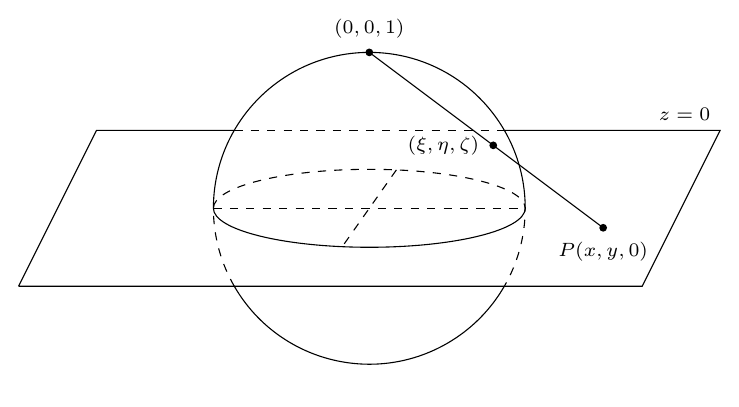
\includegraphics[width=0.90\textwidth]{stereographic_projection.png}
\end{center}
$$ v^{+} = S^2 \setminus \{(0,0,-1)\} \quad v^{-} = S^2 \setminus \{ (0,0,1) \} $$
We think of map $\phi^{-}$ as drawing a line through the point the north pole $(0,0,1)$ and $(x,y,z)$, then the output is the point where the line intersects z plane.
Similarly for $\phi^{+}$, we project from the south pole $(0,0,-1)$. We get the maps explicitly by parametrizing the line:
$$ l: (0,0,1) + t ((x_1,x_2,x_3) - (0,0,1)) =  (x_1 t,x_2 t, x_3 t-t+1) $$
$l$ intersects $x_3=0$ when $x_3t-t+1=$, thus $t = \frac{1}{(1-x_3)}$ It follows that the point of intersection is $(\frac{x_1}{1-x_3},\frac{x_2}{1-x_3},0)$
Similarly we can explicitly find $\phi^{+}$
$$ \phi_{+}: v^{+} \to \RR^2, \quad (x_1,x_2,x_3) \to (\frac{x_1}{1+x_3}, \frac{x_2}{1+x_3} )$$
$$ \phi_{-}: v^{-} \to \RR^2, \quad (x_1,x_2,x_3) \to (\frac{x_1}{1-x_3}, \frac{x_2}{1-x_3} )$$
We can find the inverses in the similar way.
Consinder points on the $z=0$ plane in $\RR^3$ $(\alpha, \beta, 0)$. We parametrize the line through this point and north pole:
$$ l: (0,0,1) + t((\alpha, \beta, 0 ) - (0,0,1)) = (\alpha t, \beta t, -t +1)$$
We need to see when are these points going to be on the sphere , i.e.
$$ (\alpha t)^2  + (\beta t)^2 + (-t +1)^2 = 1 $$
$$ \alpha^2 t^2 + \beta^2 t^2 + t^2 - 2t + 1 = 1 $$
$$ t^2 (\alpha^2 + \beta^2 +1 - \frac{2}{t} ) = 0 $$
$$ \therefore t = \frac{2}{\alpha^2 + \beta^2 +1 } $$
$$ \phi_{+}^{-1}:
\RR^2 \to v^{+} 
\quad (\alpha, \beta)  \to
( \frac{2 \alpha}{1+\alpha^2+\beta^2},
  \frac{2 \beta}{1+\alpha^2+\beta^2},
  - \frac{\alpha^2+\beta^2-1}{\alpha^2+\beta^2+1})
$$
$$ \phi_{-}^{-1}:
\RR^2 \to v^{-}
\quad (\alpha,\beta) \to
( \frac{2\alpha}{1+\alpha^2+\beta^2}, 
\frac{2\beta}{1+\alpha^2+\beta^2}, 
 \frac{\alpha^2 + \beta^2 -1}{\alpha^2+\beta^2+1} )
$$
Since we explicitly found an inverse, the function is bijection.
\newline
And it's easy to see that $\phi$ is continuous by lemma \ref{contLemma} (denom never zero)
Thus we equipped the sphere with the following atlas:
$$ A_2 = \{(v^{\pm},\phi_{\pm}) \} $$
We can check that the transition maps from $A_1$ to $A_2$ are smooth. \newline
First we check for $\varphi_3^{+} \circ \phi_{+}^{-1}$ where
$$ \varphi_3^{+}: S^2 \cap {x_3 > 0} = u_3^{+} \to D_1(0,0) \subset \RR^2 $$
$$ \phi_{+}^{-1}: \RR^2 \to v^{+} = S^2 \setminus \{ (0,0,-1) \} $$
Now, since we require that the domain of $\varphi_3^{+}$ is positive, the following is how our transition function will look like

$$\varphi_3^{+} \circ \phi_{+}^{-1}: D_1 (0,0) \to D_1(0,0), \quad \varphi_3^{+}( \phi_{+}^{-1}(x_1,x_2)) = (\frac{2x_1}{1+x_1^2+x_2^2}, \frac{2x_2}{1+x_1^2+x_2^2})$$

$$ \phi_{+}^{-1} \circ \varphi_3^{+}: D_1 (0,0) \to D_1(0,0), \quad  \phi_{+}(\varphi_3^{+}((x_1,x_2) )^{-1}) = (\frac{x_1}{1+\sqrt{1-x_1^2-x_2^2}}, \frac{x_1}{1+\sqrt{1-x_1^2-x_2^2}})$$
It is continuous componentwise and thus smooth.
Next, we list the domain and the image of the rest of transition maps.
$$\varphi_3^{-} \circ \phi_{+}^{-1}: \RR^2 \setminus \bar{D_1} (0,0) \to D_1(0,0) \setminus (0,0)$$
$$\varphi_2^{+} \circ \phi_{+}^{-1}: \RR^2 \cap \{ x_2 > 0 \} \to D_1 (0,0)$$
$$\varphi_1^{+} \circ \phi_{+}^{-1}: \RR^2 \cap \{ x_1 > 0 \} \to D_1 (0,0)$$
$$\varphi_2^{-} \circ \phi_{+}^{-1}: \RR^2 \cap \{ x_2 < 0 \} \to D_1 (0,0)$$
$$\varphi_1^{-} \circ \phi_{+}^{-1}: \RR^2 \cap \{ x_1 < 0 \} \to D_1 (0,0)$$
$$\varphi_3^{+} \circ \phi_{-}^{-1}: \RR^2 \setminus \bar{D_1} (0,0) \to D_1(0,0) \setminus (0,0)$$
$$\varphi_3^{-} \circ \phi_{-}^{-1}: D_1 (0,0) \to D_1(0,0) $$
$$\varphi_2^{+} \circ \phi_{+}^{-1}: \RR^2 \cap \{ x_2 > 0 \} \to D_1 (0,0)$$
$$\varphi_1^{+} \circ \phi_{+}^{-1}: \RR^2 \cap \{ x_1 > 0 \} \to D_1 (0,0)$$
$$\varphi_2^{-} \circ \phi_{+}^{-1}: \RR^2 \cap \{ x_2 < 0 \} \to D_1 (0,0)$$
$$\varphi_1^{-} \circ \phi_{+}^{-1}: \RR^2 \cap \{ x_1 < 0 \} \to D_1 (0,0)$$
\bibliographystyle{alpha}
\bibliography{biblio} 
\end{document}          
